\chapter{Tenciche di test e prototipazione delle interfacce}
\begin{figure}[!h]
	\centering
	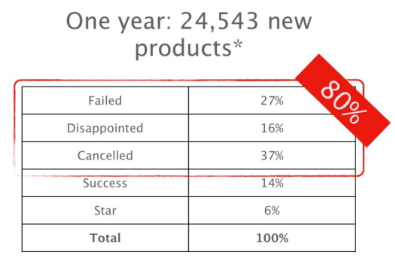
\includegraphics[scale=0.5]{immagini/Fall_mercato.png}
\end{figure}


Un prodotto \textbf{pretotipo} serve a lottare contro la legge di fallimento di mercato. Ogni anno vengono progettati e prodotti quasi 25000 nuovi prodotti l'80\% dei quali non vedrà mai la luce o non arriverà mai nelle case delle persone. Circa il 27\%
falliscono nel percorso di crescita dell'azienda, il 16\% non raggiunge le aspettative degli utenti, trattasi quindi di fallimento di mercato, e per ben il 37\% vengono cancellati durante la fase di lancio.

Del 20\% rimanente, il 14\% sono prodotti che raggiungo il mercato e ci rimangono ma
non hanno successo. \textbf{Solo il 6\% ha veramente successo}. La
\textbf{legge del fallimento di mercato sostiene che la maggior parte dei nuovi prodotti fallirà nel mercato anche se la progettazione e lo sviluppo vengono eseguite in maniera corretta e competente}.
In legge, una persona è considerata innocente fino a prova contraria, mentre nella legge di mercato, \textbf{bisogna considerare ogni prodotto come fallito fino a prova contraria}.

\section{Thoughtland, il mondo dei pensieri}
Quando si progetta un nuovo prodotto, o si ha semplicemente un'idea, ci si trova di fronte a \textbf{due grandi problemi}: il \textbf{lost in translation} e \textbf{il problema della predizione}: il primo sussiste quando l'idea è un'astrazione soggettiva, qualcosa che si può immaginare o visualizzare in testa. Nel momento in cui si prova a comunicarla a qualcun altro però, si incontra un problema
di traduzione, specialmente quando l'idea è nuova ed è diversa da qualsiasi altra cosa
abbia visto l'interlocutore.

Il modo in cui si immagina un nuovo prodotto ed i suoi usi può essere completamente diverso da come gli altri lo immaginano a loro volta. Si può ovviare utilizzando \textbf{termini noti}, infatti, è molto difficile veicolare il modello concettuale all'utente. L'altro problema è conosciuto come il \textbf{problema della predizione}: anche se la comprensione astratta dell'idea che l'interlocutore ha è molto vicina alla propria, egli in quanto essere umano è molto \textbf{scarso per sua natura} nel prevedere se essa potrebbe essere di suo gradimento o meno.

\pagebreak

\section{Thoughts without data are just opinions}

\begin{flushleft}
	\textit{I pensieri senza dati sono solo opinioni.}
\end{flushleft}

Questa è una delle più importanti frasi da tenere presente quando si pensa di lanciare nuovi oggetti o idee nel mercato, anche se è spesso sottovalutata.

I falsi positivi possono portare a credere che l'idea sia immune alla legge del
fallimento di mercato, e quindi a investire troppo e presto in un prodotto che probabilmente fallirà.

I falsi negativi possono invece spaventare e portare a non concedere una chance all'idea, finendo per scartare prematuramente il prossimo Twitter, Google o Tesla.

Per poter minimizzare la possibilità di ottenere falsi positivi o negativi è necessario \textbf{uscire dal Thoughtland}, quindi dal mondo delle idee astratte e delle opinioni, e \textbf{muoversi verso l'Actionland}, dove si usano \textbf{artefatti} per collezionare dati e osservare le azioni degli utenti. Nel primo caso si usano le domande o questionari per poter ottenere informazioni sul prodotto
che si andrà a sviluppare, col rischio di collezionare opinioni poco utili e magari fuorvianti, nel secondo caso, mediante artefatti, si fanno svolgere azioni agli utenti al fine di raccogliere dati.

I prodotti del Thoughtland sono: \textbf{idee, domande e opinioni}. Quelli dell'Actionland sono \textbf{artefatti}, \textbf{azioni} e \textbf{dati}.

\begin{figure}[!h]
	\centering
	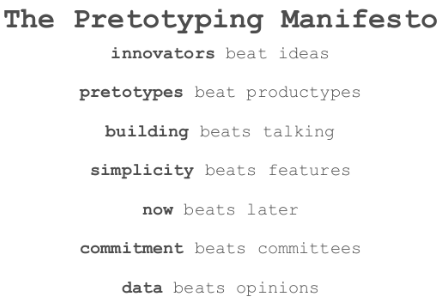
\includegraphics[scale=0.6]{immagini/Manifesto.png}
\end{figure}

\section{Pretotype vs Prototype}
I prototipi aiutano a fallire in fretta, ma spesso non abbastanza in fretta o non abbastanza economicamente.

Più si investe in un'idea e \textbf{più diventa difficile lasciarla morire} e ammettere che era sbagliata, anzi tendenzialmente, una volta ottenuto un buon prototipo che funziona, è facile portarlo avanti investendovi ancora denaro e tempo, pensando che l'aggiunta di funzionalità e features sia la risposta per renderlo vincente.

Molto spesso i prodotti lanciati sul mercato non sono altro che prototipi andati troppo oltre. \textbf{Tra il mondo delle idee astratte e i prototipi funzionanti}, si collocano i \textbf{pretotypes}.

\textbf{Un pretotipo è un semplice mockup del prodotto che si vorrebbe sviluppare} ed è utile per ottenere sia informazioni d'uso che di mercato e, specialmente, per poter prendere decisioni su cosa fare e su cosa non fare.

La \textbf{principale differenza} tra un pretotipo e un prototipo è l'\textbf{investimento}: un \textbf{pretotipo costa molto meno} sia in termini di tempo che in termini di denaro, e consente di fallire in fretta o nel caso, poiché lascia un ampio spazio di manovra, di apportare modifiche.

\pagebreak

\begin{figure}[!h]
	\centering
	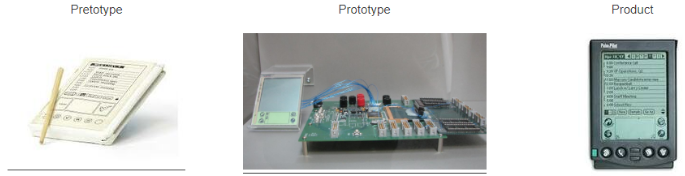
\includegraphics[scale=0.65]{immagini/Pre_prot.png}
\end{figure}

Il \textbf{pretotyping} ha l'obiettivo di aiutare a:

\begin{itemize}
	\item \textbf{Identificare le funzionalità chiave} del nuovo prodotto.
	\item Decidere \textbf{quali} di queste possono o dovrebbero essere \textbf{inserite nel mockup}.
	\item Usare i mockups per il \textbf{test sistematico} e contemporaneamente \textbf{collezionare feedback e dati d'uso}.
	\item Analizzare i dati raccolti per \textbf{determinare il prossimo passo da compiere}.
\end{itemize}

I \textbf{sette pilastri del Pretotyping} sono:

\begin{enumerate}
	\item \textbf{Obbedire alla Legge del Fallimento di Mercato}.
	\item \textbf{Assicurarsi di star costruendo il prodotto giusto}.
	\item \textbf{Non perdersi in chiacchiere, idee o opinioni}.
	\item \textbf{Fidarsi solo dei propri dati, \textbf{TRUST YODA: Your Own DAta}}.
	\item \textbf{Fare pretotyping}.
	\item \textbf{Parlare con i numeri e con i fatti}.
	\item \textbf{Pensare globalmente e non localmente}.
\end{enumerate}

\section{Flusso del Pretotyping}

I \textbf{cinque step} per produrre un buon pretotipo sono i seguenti:

\begin{enumerate}
	\item \textbf{Isolare l'assuzione chiave}: qual è la assunzione o funzionalità chiave dell'idea che, se falsa, ne minerebbe la validità?
	\item \textbf{Scegliere un tipo di pretotype}: quale tipo di pretotyping permette di isolare e testare al meglio le funzionalità chiave?
	\item \textbf{Fare ipotesi di mercato}: quante e quali tipi di persone utilizzeranno il pretotipo? Come lo utilizzeranno? Sarebbe possibile ipotizzare le percentuali di un determinato utilizzo?
	\item \textbf{Testare il pretotype}: mettere il pretotipo nel mondo reale e vedere quante persone sono interessate e quante ci interagiscono. Bisogna partire dal basso, un passo alla volta.
	\item \textbf{Imparare, rifinire, hypozoom}: valutare i risultati, rifinire il pretotipo con i nuovi dati, e se l'ipotesi ha retto, decidere quali altre situazioni testare per ottenere man mano una \textbf{visione completa: hypozooming}.
\end{enumerate}

\pagebreak

\section{Tipi di Pretotyping}
Andiamo ad analizzare alcuni tipi di pretotyping.
\begin{itemize}
	\item Una \textbf{Fake Door} è un marketing entry point per un prodotto che ancora \textbf{non esiste} e può essere utilizzata per \textbf{pubblicizzare} un servizio non ancora pronto e misurare l'interesse degli utenti.

	      È un buon modo per capire se l'oggetto che si vuole sviluppare può avere successo o meno, spendendo pochissimo e quindi, in caso di fallimento, avere un basso impatto economico, inteso sempre sia in termini di denaro che di tempo. Si può usare
	      questo tipo di pretotyping \textbf{quando l'idea può essere descritta in poche e semplici parole}, senza possedere nulla di fisico o materiale.

	      \begin{figure}[!h]
		      \centering
		      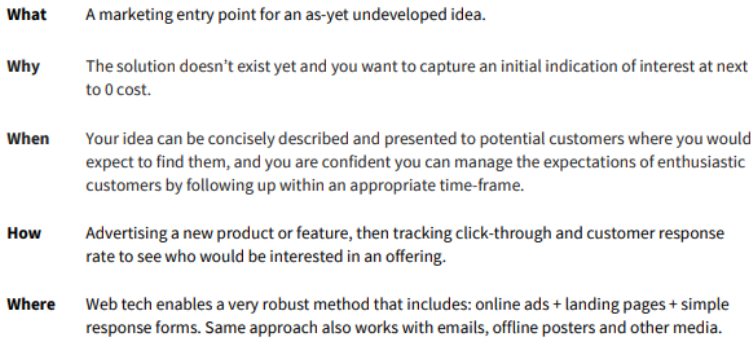
\includegraphics[scale=0.42]{immagini/Fake_door.png}
	      \end{figure}

	\item Si parla di \textbf{Mechanical Turk} quando ci si riferisce ad un oggetto che riesce, nel suo utilizzo, a trasmettere l'esperienza del prodotto finale ad un utente, senza che sia stato sviluppato. Un meachanical turk usa solo man power. È molto utilizzato per sperimentare l'uso e la reale applicabilità di software e algoritmi molto costosi per essere implementati.

	      \begin{figure}[!h]
		      \centering
		      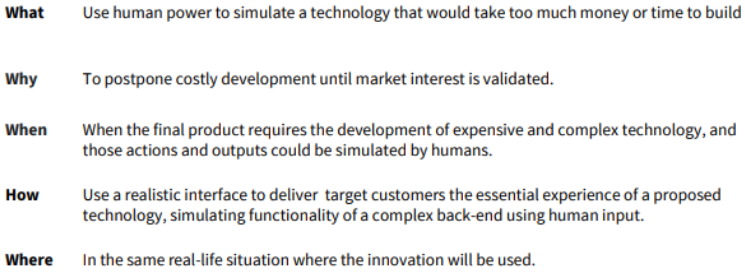
\includegraphics[scale=0.42]{immagini/Mechanical_turk.png}
	      \end{figure}

	\item Un \textbf{Impersonator} è un pretotipo che riesce a far sperimentare un'esperienza realistica all'utente in modo estremamente economico e con un lavoro minimo dietro. Consente cioè di
	      far vivere l'esperienza esattamente come se il prodotto fosse finito e pronto per essere lanciato.

	      \begin{figure}[!h]
		      \centering
		      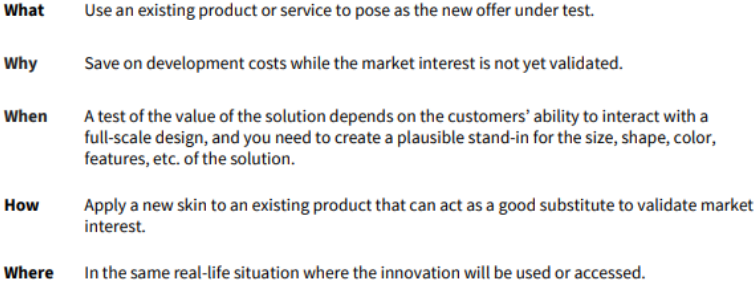
\includegraphics[scale=0.42]{immagini/Impersonator.png}
	      \end{figure}

	      \pagebreak

	\item Un \textbf{Pinocchio} è un pretotipo \textbf{chiaramente falso}, serve per veicolare un messaggio così distante dalla realtà attuale che è faticoso e difficile da spiegare in altri linguaggi naturali. È usato molto spesso per testare l'interesse e il possibile uso di prodotti innovativi e non ancora lanciati da nessuno, nemmeno in maniera simile, sul mercato.

	      \begin{figure}[!h]
		      \centering
		      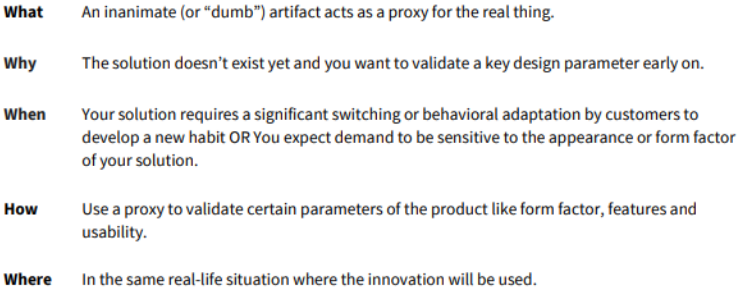
\includegraphics[scale=0.5]{immagini/Pinocchio.png}
	      \end{figure}

	\item Con \textbf{One Night Stand} si indica una \textbf{tecnica di veicolazione} di un pretotipo. Consiste di un \textbf{market test}.
	      Viene usato insieme ad un'altra tecnicha di pretotyping per veicolare meglio il messaggio a una certa cerchia di persone.

	      \begin{figure}[!h]
		      \centering
		      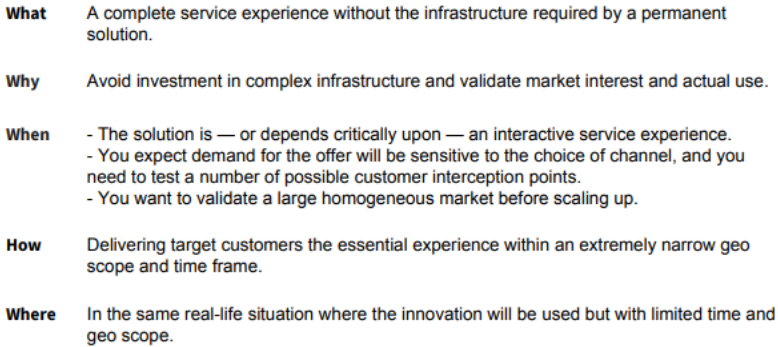
\includegraphics[scale=0.5]{immagini/One_night_stand.png}
	      \end{figure}


	\item Un \textbf{Facade} è una sorta di Impersonator ma è usato per dare un'immagine dell'azienda e non del prodotto stesso. Viene sfruttato spesso per promuovere servizi.

	      \begin{figure}[!h]
		      \centering
		      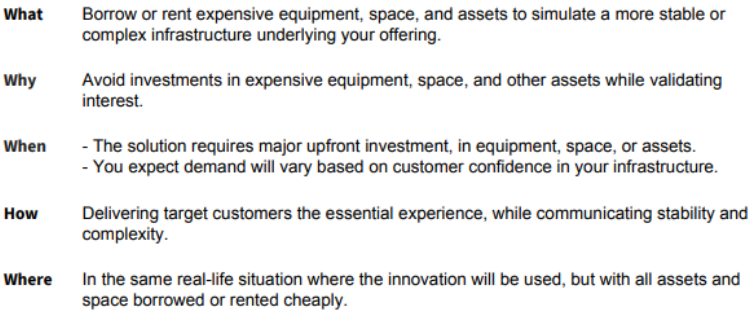
\includegraphics[scale=0.5]{immagini/Facade.png}
	      \end{figure}

\end{itemize}

\pagebreak

\section{Minimum Viable Product}

Dopo varie fasi di pretotyping e aver accumulato sicurezze sufficienti circa il successo del prodotto, lo step successivo è produrre il \textbf{Minimum Viable Product}, cioè la \textbf{versione minimale del prodotto contenente solo ed esclusivamente le features che si sono pretotipate attraverso la fase precedente}.
Non si ha ancora per le mani un prodotto definitivo besì un qualcosa di \textbf{vendibile}, in modo da ottenere del ricavo e dell'utile, che se sufficiente, permetterebbe la produzione definitiva del prodotto.

\begin{figure}[!h]
	\centering
	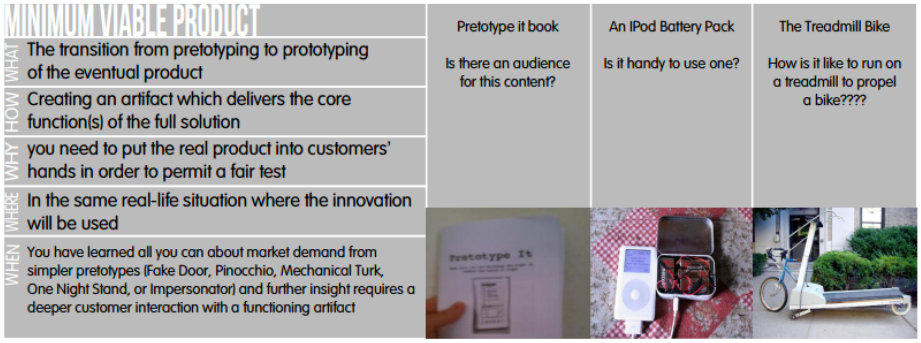
\includegraphics[scale=0.5]{immagini/MVP.png}
	\caption{Minimum Viable Product.}
	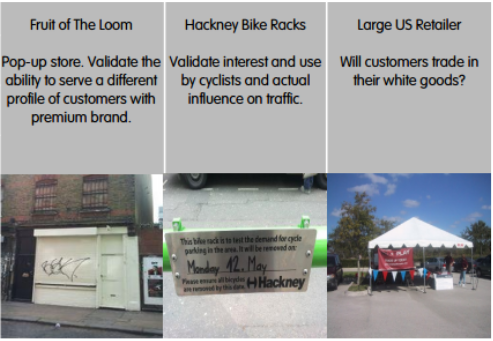
\includegraphics[scale=0.4]{immagini/ONS.png}
	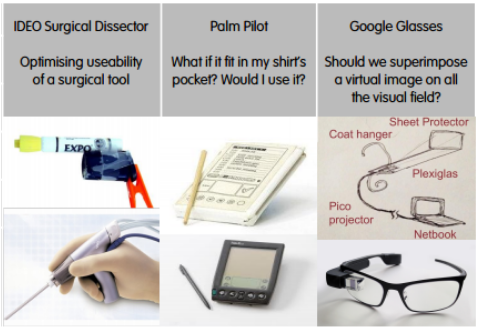
\includegraphics[scale=0.4]{immagini/Pnocc.png}
	\caption{A sinistra esempi di one night stands e a destra esempi di pinocchio.}
	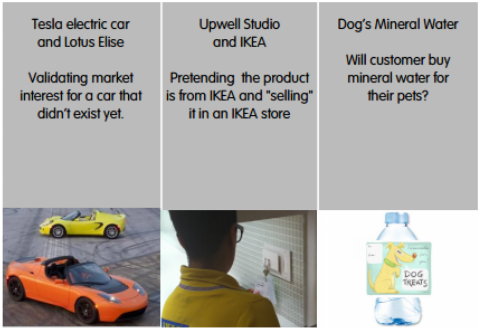
\includegraphics[scale=0.6]{immagini/Imp.png}
	\caption{Esempi di Impersonator.}
\end{figure}

\pagebreak

